\section{Introduction}
%I love image analysis and stuff. But sometimes it just sucks. Especially these times when you're supposed to write a bloody report about stuff you probably don't understand and will just bable like you do. So enjoy:
%\\\\
%Once upon a time there was a person filming another person. The movie had to be just right for it to be rewatched year after year with many laughs and tears to follow. But there was a problem. The other person, the one being filmed, was moving very fast here and there. The person filming was having trouble getting the pan, tilt and zoom of the camera correct or else something might be missed.

%Frigöra sig från linsen
%att både ha kakan och äta upp den
%best of both worlds

Tracking a plethora of moving objects, such as an ongoing soccer game, with a mechanical PTZ can be a somewhat daunting task. With things happening all over the surveyed scene and the sometimes significant response time of actuators in the PTZ-camera, there is a real possibillity that the camera is pointed in the ''wrong direction at the wrong time'', see fig. \ref{fig:problem}.

\begin{figure}[H]
	\centering
	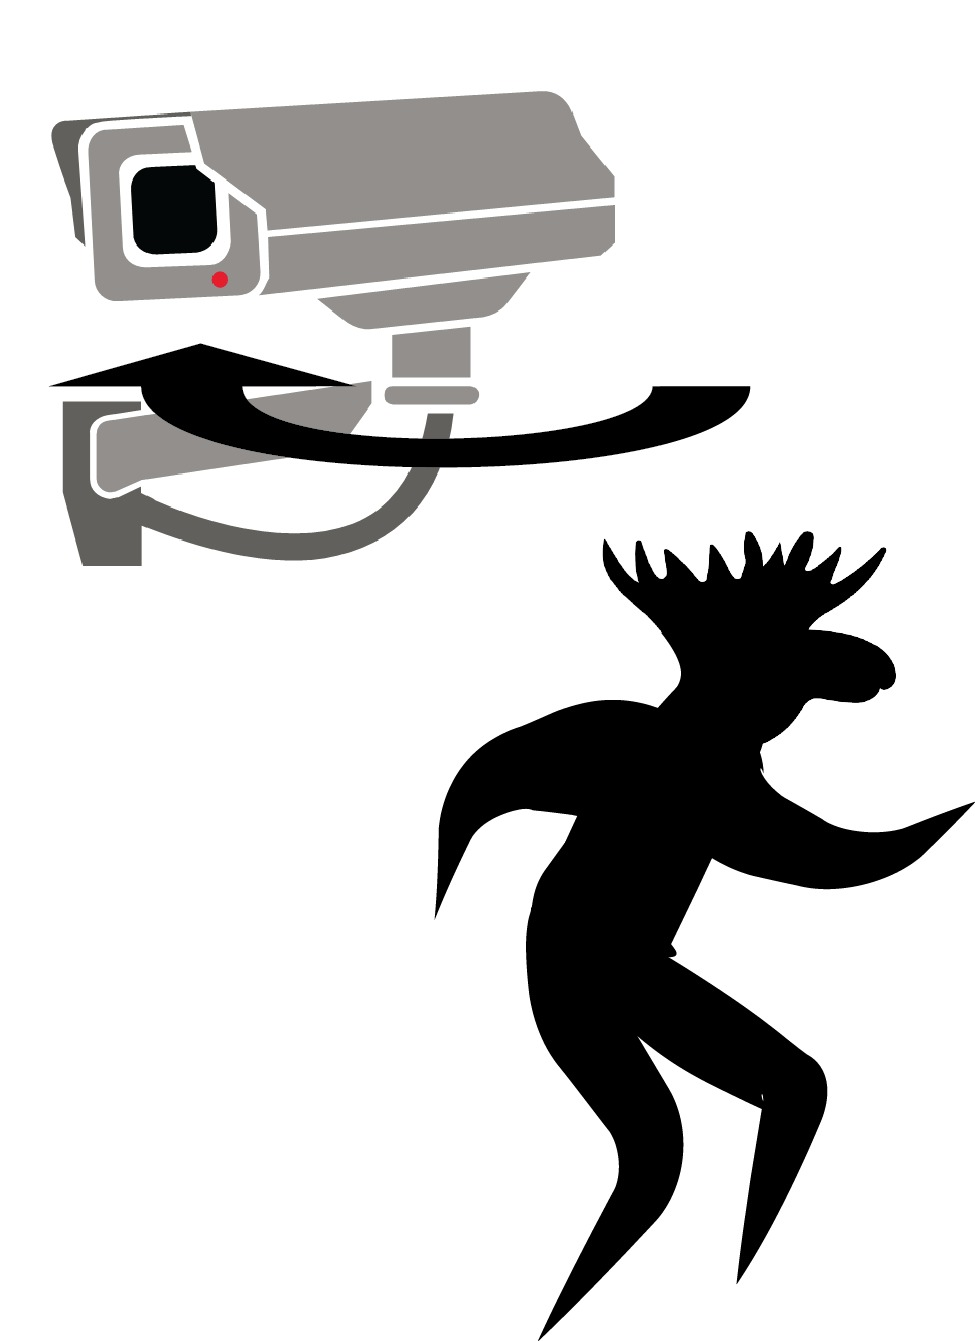
\includegraphics[width=0.3 \textwidth]{../results/PTZ_problem.jpg}
	\caption{A panable camera looking in the wrong direction, therby not noticing a moose sneaking by.}
	\label{fig:problem}
\end{figure}

In this project we investigate another method, where multiple stationary cameras are used to cover the entire scene under surveillance, and then produce the PTZ-motion in software by panoramic stitching and virtual cameras.
